\documentclass[10pt]{article}
\usepackage[T1]{fontenc}
\usepackage{lmodern,amsmath,amssymb,graphicx,hyperref}
\usepackage[margin=.74in]{geometry}
\setlength{\parindent}{0pt}\setlength{\parskip}{7pt}
\begin{document}
\begin{center}{\Large Actual off-diagonal support and even-moment controls}\\[4pt]
Local continuation --- 15 November 2026\end{center}
\textbf{Result.} The proposed off-diagonal coefficient prediction is confirmed:
the actual odd right-factor first coefficient is $-8/9$. For every $a\ge3$,
an actual left factor equal to $C(2)$ makes the same odd label jointly active.
Thus matching-port first-jet cancellation cannot justify deleting whole odd
modes. A separate exact even-moment formula supplies nonzero positive controls
[pcc:unverified].

\textbf{Frozen right-only fixture.} Set $u=2$, $i=0$, $k=2$, residue $r=0$,
column $y=2$ and moment index $b=1$. Use node $-1$ and multiplicities one at
anchor $+1$, zero elsewhere. The retained bit condition holds. For every
$a\ge2$, the actual coefficient proof yields
\[
 [Z^1]R_{(0,1),2}(Z)=-\frac89.
\]
This includes the original frozen $a=2$ fixture [pcc:unverified].

\textbf{Derived quantities.} The actual normalized node first coefficient is
$-1/3$, derived from firstJet and diagonalJet with a proved nonzero common
jetScalar. The actual geometric $H^1Z^0$ coefficient is $16/3$. The normalized
right coefficient is therefore
\[
 \frac12\left(-\frac13\right)\left(\frac{16}{3}\right)=-\frac89.
\]
The proof reduces the actual retained correction and anchor products, rather
than supplying these numbers as favorable witnesses [pcc:unverified].

\textbf{Joint witness and fixture correction.} When $a=u=2$, each residue
class contains only its base port; its quotient is zero, so higher left
moments vanish. The original fixture is therefore a right-factor control,
not evidence of joint mode activity. For every $a\ge3$, choose actual row
port $x=4$ and column port $y=2$. The source proves
\[
 L_{4,(0,1)}=C(2)\ne0,\qquad
 [Z^1]R_{(0,1),2}=-8/9\ne0.
\]
This is a genuine jointly active odd-mode witness for an infinite family of
outer grid sizes. It is not a runtime or rank lower bound
[pcc:unverified].

\textbf{Evidence.} Accepted084 contains392 local theorem statements including
parent384, eight new, exit0 and no warnings. Receipt042/data1c1f5f pin the exact
source, raw output and exit. Central printed dependencies are standard.
Failed082 and083 are retained. The local evidence is outside shared
Transport53/57/fresh, unsigned and defaultnot\_covered [pcc:unverified].
\newpage
\begin{center}{\Large Even positive controls and the next valuation test}\end{center}
\textbf{Exact even coefficient.} Let $i<u\le a$, use the same single-anchor
profile at $i$, a matching residue port $r$, and any admissible even moment
$2b<k$. The proof derives from the actual finite geometric sum
\[
 [H^{2b}]\sum_{n<k}(c^2H^2)^n=c^{2b},\qquad
 c=\frac{2^u}{2^i}.
\]
Actual numerator and normalization then give
\[
 [Z^1]R_{(r,2b),r}=\bigl(2^{2b}\bigr)^{-1}c^{2b}\ne0.
\]
This is a positive control on the actual right expression, not an assumed
support count [pcc:unverified].

\textbf{Separate acceptance.} Accepted086 contains397 statements including
parent392, five new, exit0 without warnings or sorryAx. Receipt043 separately
pins the source and raw outputs. Warning-bearing085 passed compilation but
is preserved as that earlier status;086 replaces the deprecated lemma without
suppression. Central printed dependencies are standard [pcc:unverified].

\begin{center}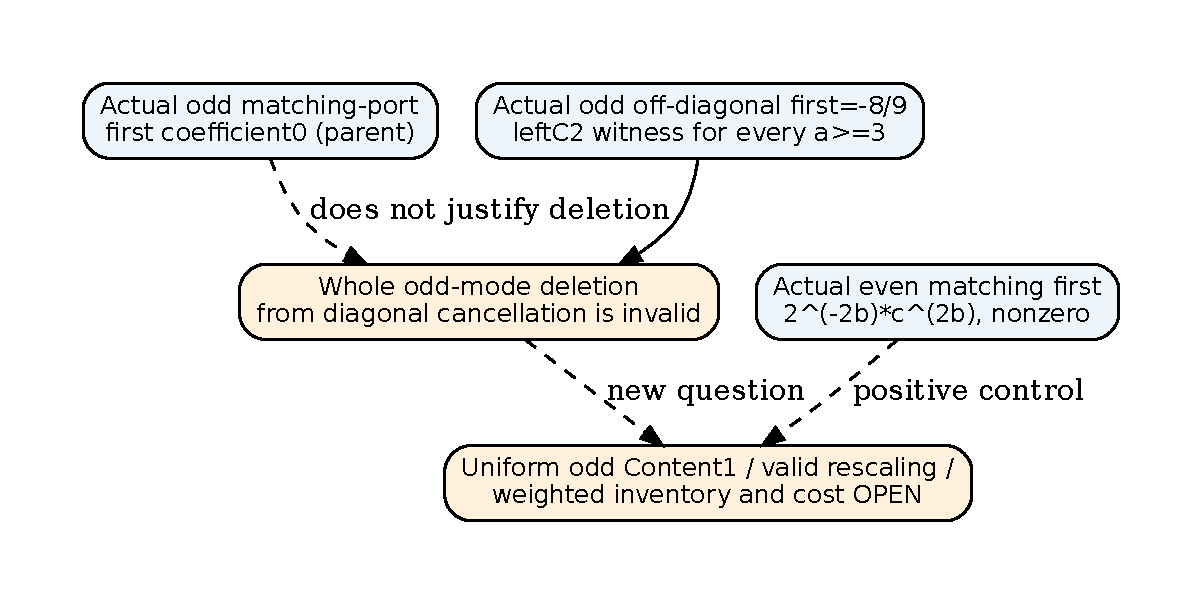
\includegraphics[height=2.7in]{support-controls-dependencies-001.pdf}\end{center}

\textbf{Decision.} Reject deleting odd modes solely because their matching-port
first coefficient vanishes. Neither a nonzero rational coefficient nor this
joint-support counterexample rules out additional uniform two-adic
divisibility. That is a different quantified property and requires every
column and every coefficient, with actual label/mask conditions
[pcc:unverified].

\textbf{Next acceptance target.} PROTOCOL-013.md asks for an exact proof or
counterexample to Content1 of every actual odd right factor in the single-anchor
profile. Review prior parity, binomial and valuation sources first. If proved,
construct right/2 and left times2 as integral rationals before finite-ring
reduction, preserving the actual product and residual; do not invert two in
the finite ring. Charge all precision, preparation and bit costs
[pcc:unverified].

\textbf{Remaining scope.} A single-anchor profile does not automatically meet
original all-node schedule and child-degree admission. All $2^u k$ labels,
original packet and full public expected-cost interfaces remain charged or
open. No native timing, scaling, paid/cloud or attack campaign was run.
Protected histories and parent immutable bytes remain exact;watcher paused
[pcc:unverified].
\end{document}
